%%% The following code is based on the work of Nicolas Normand
% used for his paper for WCNC 2010 regarding "Erasure Coding with
% the Finite Radon Transform"

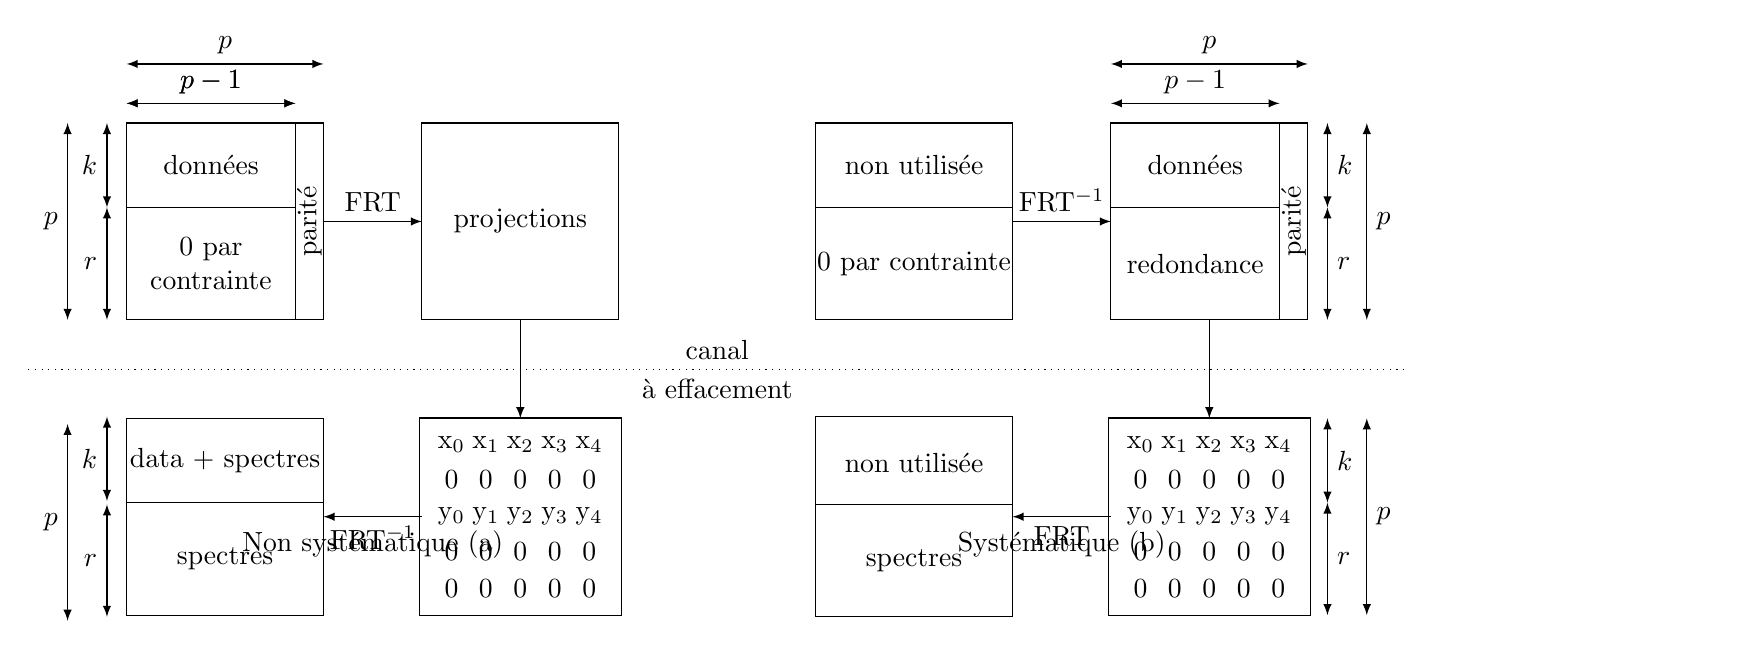
\begin{tikzpicture}[
	y=1cm,
	x=1cm,
	scale=1] {

\def\scale{2.8}
\def\r{4/\scale}
\def\k{3/\scale}
\def\one{1/\scale}
\def\pm{6/\scale}
\def\p{7/\scale}
% initial rectangle (non systématique image space)
\path[fill=white,draw=black] (0,\r)
    rectangle + (\pm,\k)
    node[midway]{données};
\path[fill=white,draw=black, align=center] (0,0)
    rectangle + (\pm,\r)
    node[midway]{0 par \\ contrainte};
\path[fill=white,draw=black] (\pm,0)
    rectangle + (\one,\p)
    node[midway,rotate=90]{parité};
\draw[latex-latex] (-.75,0) -- node[left] {$p$} +(0,\r+\k);
\draw[latex-latex] (-.25,0) -- node[left] {$r$} +(0,\r);
\draw[latex-latex] (-.25,\r) -- node[left] {$k$} +(0,\k);
\draw[latex-latex] (0,\p+.25) -- node[above] {$p-1$} +(\pm,0);
\draw[latex-latex] (0,\p+.75) -- node[above] {$p$} +(\p,0);

% rectangle below (non systématique Ghosted image)
\path[fill=white,draw=black] (0,-\p/2)
    rectangle + (\p,-\k)
    node[midway]{data $+$ spectres};
\path[fill=white,draw=black,align=center] (0,-\p/2-\k)
    rectangle + (\p,-\r)
    node[midway]{spectres};

%rectangle on the right below (non systématique Ghosted Radon space)
   \matrix [draw, column sep=-0.14cm]
    at (3*\p-\p,-\p)
    {
	\node (a) {x$_{0}$}; & \node {x$_{1}$}; & \node {x$_{2}$}; &
	\node {x$_{3}$}; & \node {x$_{4}$}; \\
	\node (b) {$0$}; & \node {$0$}; & \node {$0$}; &
	\node {$0$}; & \node {$0$}; \\
	\node (c) {y$_{0}$}; & \node {y$_{1}$}; & \node {y$_{2}$}; &
	\node {y$_{3}$}; & \node {y$_{4}$}; \\
	\node (d) {$0$}; & \node {$0$}; & \node {$0$}; &
	\node {$0$}; & \node {$0$}; \\
	\node (e) {$0$}; & \node {$0$}; & \node {$0$}; &
	\node {$0$}; & \node {$0$}; \\
    };

% top right rectangle (non systématique Radon space)
\path[fill=white,draw=black] (3*\p/2,0)
    rectangle + (\p,\p)
    node[midway]{projections};

% link
%\draw[dashed,-latex] (5*\p/2,\p/2) -- node[above]{Alg.2}
%    node[below]{Row-Solving} +(\p,0);

% double right rectangle (systématique image space)
\path[fill=white,draw=black] (5*\p,\r)
    rectangle + (\pm,\k)
    node[midway]{données};
\path[fill=white,draw=black, align=center] (5*\p,0)
    rectangle + (\pm,\r)
    node[midway]{redondance};
\path[fill=white,draw=black] (5*\p+\pm,0)
    rectangle +(\one,\p)
    node[midway,rotate=90]{parité};

% double right rectangle below (systématique Ghosted image space)
   \matrix [draw, column sep=-0.14cm]
    at (11*\p/2,-\p)
    {
	\node (a) {x$_{0}$}; & \node {x$_{1}$}; & \node {x$_{2}$}; &
	\node {x$_{3}$}; & \node {x$_{4}$}; \\
	\node (b) {$0$}; & \node {$0$}; & \node {$0$}; &
	\node {$0$}; & \node {$0$}; \\
	\node (c) {y$_{0}$}; & \node {y$_{1}$}; & \node {y$_{2}$}; &
	\node {y$_{3}$}; & \node {y$_{4}$}; \\
	\node (d) {$0$}; & \node {$0$}; & \node {$0$}; &
	\node {$0$}; & \node {$0$}; \\
	\node (e) {$0$}; & \node {$0$}; & \node {$0$}; &
	\node {$0$}; & \node {$0$}; \\
    };

% double double right rectangle (systématique Radon space)
\path[fill=white,draw=black,align=center] (7*\p/2,\r)
    rectangle + (\p,\k) node[midway]{non utilisée};
\path[fill=white,draw=black,align=center] (7*\p/2,0)
    rectangle + (\p,\r) node[midway]{0 par contrainte};

% parameters below
\draw[latex-latex] (6*\p+0.75,-3*\p/2) -- node[right] {$p$} +(0,\p);
\draw[latex-latex] (6*\p+0.25,-3*\p/2) -- node[right] {$r$} +(0,\r);
\draw[latex-latex] (6*\p+0.25,-3*\p/2+\r) -- node[right] {$k$} +(0,\k);

% double double right rectangle below (systématique Ghosted Radon space)
\path[fill=white,draw=black] (7*\p/2,-\p+0.1)
    rectangle + (\p,\k+0.1) node[midway]{non utilisée};
\path[fill=white,draw=black,align=center] (7*\p/2,-\p-\k-0.2)
    rectangle + (\p,\r)
    node[midway]{spectres};

\draw[latex-latex] (6*\p+0.75,0) -- node[right] {$p$} +(0,\r+\k);
\draw[latex-latex] (6*\p+0.25,0) -- node[right] {$r$} +(0,\r);
\draw[latex-latex] (6*\p+0.25,\r) -- node[right] {$k$} +(0,\k);
\draw[latex-latex] (0,\p+.25) -- node[above] {$p-1$} +(\pm,0);
\draw[latex-latex] (5*\p,\p+.25) -- node[above] {$p-1$} +(\pm,0);
\draw[latex-latex] (5*\p,\p+.75) -- node[above] {$p$} +(\p,0);
\draw[latex-latex] (-.75,-\p-\k-0.25) -- node[left] {$p$} +(0,\r+\k);

\draw[-latex] (\p,\p/2) -- node[above] {FRT} + (\p/2,0);
\draw[latex-] (\p,-\p) -- node[below]{FRT$^{-1}$}
    node[below=\p/1.7]{Non systématique (a)} + (\p/2,0);

\draw[-latex] (9*\p/2,\p/2) -- node[above] {FRT$^{-1}$} + (\p/2,0);
\draw[latex-] (9*\p/2,-\p) -- node[below] {FRT}
    node[below=\p/1.7]{Systématique (b)} + (\p/2,0);

\draw[-latex] (11*\p/2,0) -- + (0,-\p/2);
\draw[-latex] (\p+\p,0) -- + (0,-\p/2);

\draw[latex-latex] (-0.25,-\k-\p-0.2) -- node[left] {$r$} +(0,\r);
\draw[latex-latex] (-.25,-\p+0.2) -- node[left] {$k$} +(0,\k);

\draw[dotted] (-\p/2,-\p/4) -- 
    node[above] {canal} node[below] {à effacement} + (7*\p,0);
\draw (8*\p, 0) -- node {} (8*\p,0);
}\end{tikzpicture}

